
%*******************************************************************************
%*********************************** First Chapter *****************************
%*******************************************************************************
%!TEX root = 0.main.tex

\section{Improving Deep Sphere}

\subsection{Definitions and basic results}

Let us recall some basic definitions necessary for this chapter:
\vspace{0.5cm}
\begin{definition}{}(Heat Kernel Graph Laplacian Matrix)\\
	\label{def:Heat Kernel Graph Laplacian Matrix}
	\text{For a sampling $\{x_i\in\mathcal S_2\}_{i=0}^{n-1}$ of the sphere we define the \textbf{matrix} }
	$$\mathbf L_n^t:\quad(\mathbf L_n^t)_{ij} := \frac{1}{n}\left[ \sum_{i=0}^{n-1} e^{-\frac{||x_i-x_j||^2}{4t}}\left(f(x_j)-f(x_i)\right)\right]$$
	where $||\cdot||$ is the Euclidean norm in the ambient space $\mathbb R^N$.
\end{definition}
\vspace{0.5cm}
\begin{definition}{}(Heat Kernel Graph Laplacian operator)\\
	\label{def:Heat Kernel Graph Laplacian operator}
	\text{For a sampling $\{x_i\in\mathcal S_2\}_{i=0}^{n-1}$ of the sphere we define the \textbf{operator} }
	$$L_n^t:\quad(L_n^tf)(y) := \frac{1}{n}\left[ \sum_{i=0}^{n-1} e^{-\frac{||x_i-y||^2}{4t}}\left(f(y)-f(x_i)\right)\right]$$
\end{definition}
\vspace{0.5cm}
\begin{definition}{}(Functional approximation to the Laplace-Beltrami operator)\\ \label{eq: my L^t}
	\label{def:Functional approximation to the Laplace-Beltrami operator}
	$$L^t:\quad L^tf(y) := \int_{\mathcal S_2}e^{-\frac{||p-x||^2}{4t}}\left(f(y)-f(x)\right)d\mu(x)$$
	\text {where $\mu(x)$ is the uniform measure on the sphere}
\end{definition}
\vspace{0.5cm}

\begin{prop}(Hoeffding's inequality)\\
	Let \(X_{1}, \ldots, X_{n}\) be independent identically distributed random variables, such that
	\(\left|X_{i}\right| \leqslant K .\) Then
	
	$$
	\mathbb P\left\{\left|\frac{\sum_{i} X_{i}}{n}-\mathbb{E} X_{i}\right|>\epsilon\right\}<2 \exp \left(-\frac{\epsilon^{2} n}{2 K^{2}}\right)
	$$
	\label{theo:Hoeffding}
\end{prop}
\subsection{Adapting Belkin's setting to HEALPix sampling}

[Review of Belkin et al's proof: the 2 steps] 

Belkin et al. in \cite{Belkin:2005:TTF:2138147.2138189} prove the following pointwise convergence result for the Heat Kernel Graph Laplacian operator built on a random sampling on any $k$-dimensional compact smooth manifold $\mathcal M$ embedded in some euclidean space $\mathbb R^N$:
\vspace{0.5cm}
\begin{theorem}{(Theorem 3.1 of \cite{Belkin:2005:TTF:2138147.2138189})}\\
	\label{theo:Belkin pointwise convergence}
	Let $\mathcal M$ be a $k$-dimensional compact smooth manifold embedded in some euclidean space $\mathbb R^N$. Let the data points $x_1, ... x_n$ be sampled form a uniform distribution on the manifold $\mathcal M$. Set $t_n=n^{-\frac{1}{k+2+\alpha}}$, for any $\alpha>0$ and let $f\in\mathcal C_\infty(\mathcal M)$. Then:
	
	$$\forall \epsilon>0\quad \mathbb{P}\left[\left|\frac{1}{t}\frac{1}{(4 \pi t)^{k/2}}L_{n}^{t_n} f(p)-  \frac{1}{|\mathcal M|}L^{t_n} f(p)\right|>\epsilon\right] \xrightarrow{n\to\infty} 0$$
\end{theorem}
\vspace{0.5cm}

In this section we'll prove a similar result but on the specific case of the manifold $\mathcal M$ being the 2-Sphere $\mathcal S_2$ where the points $x_1, ..., x_n$ are not sampled form a random distribution on the manifold, but are defined by the HEALPix sampling defined in section \ref{sec:HEALPix}. Since our result is similar to theorem \ref{theo:Belkin pointwise convergence}, it is useful to first review the proof of theorem \ref{theo:Belkin pointwise convergence} before stating the main result of this section.
\begin{proof}
The first step to prove theorem \ref{theo:Belkin pointwise convergence} is observing that for any fixed $t>0$, any fixed function $f$ and a fixed point $y\in\mathcal S_2$,  the Heat Kernel Graph Laplacian $L_n^t$ is an unbiased estimator for the Functional Approximation of the Laplace-Beltrami $L^t$. In other words, $L_n^tf(y)$ is the empirical average of $n$ i.i.d. random variables $X_i= e^{-\frac{||x_i-y||^2}{4t}}\left(f(y)-f(x_i)\right)$ with expected value corresponding to $L^tf(y)$. Thus, for the strong law of large numbers we have that
\begin{equation}
\label{eq:convergence in probability}
\lim_{n\to\infty}L_n^tf(y) = L^t(y)
\end{equation}
where the limit is in the sense of the strong law of large numbers.
The core of \cite{Belkin:2005:TTF:2138147.2138189} is the proof, that we will not discuss, of the following proposition:

\begin{prop} Under the same hypothesis of theorem \ref{theo:Belkin pointwise convergence},
	$$\frac{1}{t}\frac{1}{(4\pi t)^{k/2}} L^tf(y) \xrightarrow{t\to 0 } \frac{1}{|\mathcal M|}\triangle_{\mathcal M}f(y)$$
	\label{prop:3}
\end{prop}

Thanks to Proposition \ref{prop:3} and equation \ref{eq:convergence in probability}, a straightforward application of Hoeffding's inequality (Proposition \ref{theo:Hoeffding}) with $K=\frac{1}{t}\frac{1}{(4\pi t)^{k/2}}$ leads to

\begin{equation}
	\label{eq:hoeffding applied}
	\mathbb{P}\left[\frac{1}{t(4 \pi t)^{k / 2}}\left|L_{n}^{t} f(y)-\mathbb{E} L_{n}^{t} f(y)\right|>\epsilon\right] \leq 2 e^{-1 / 2 \epsilon^{2} n t(4 \pi t)^{k / 2}}
\end{equation}

We want the right hand side of equation \ref{eq:hoeffding applied} to go to $0$ for $n\to\infty, t\to0$ at the same time. For this to happen, we need to find a sequence $(t_n)$ such that 
$$\begin{cases}
t_n\xrightarrow{n\to\infty}0\\
2 e^{-1 / 2 \epsilon^{2} n t_n(4 \pi t_n)^{k / 2}}\xrightarrow{n\to\infty}0\\
\end{cases}$$

By fixing $t_n=n^{-\frac{1}{k+2+\alpha}}$, for any $\alpha>0$, it is easy to check that $-1 / 2 \epsilon^{2} n t_n(4 \pi t_n)^{k / 2}\xrightarrow{n\to\infty}+\infty$ concluding the proof.

\end{proof}

Now that we presented the proof of theorem \ref{theo:Belkin pointwise convergence}, we can observe that in order to adapt the proof to the case of the sphere with the HEALPix sampling  two are the key elements of the proof that we need to modify. First, due to the deterministic nature of the HEALPix sampling on the sphere, we need to prove that for any fixed $t>0$, any fixed function $f$ and any point $y\in\mathcal S_2$ $$\left|L_n^tf(y)-L^tf(y)\right|\xrightarrow{n\to \infty} 0$$ without relying on the strong law of large numbers. Once proven such result, we need to construct an inequality of the kind

$$\left|\frac{1}{4\pi t^2}\left(L_n^tf(x) - L^tf(x)\right)\right|\leq C(t, n)\xrightarrow[n\to \infty]{t\to 0}0$$

to then use Proposition \ref{prop:3} to prove our main result:
\vspace{1cm}
\begin{theorem}
	For a sampling $\{x_i\in\mathcal S_2\}_{i=0}^{n-1}$ of the sphere, for all $f: \mathcal S_2 \rightarrow \mathbb R$ Lipschitz, for all $y\in\mathcal S_2$, the rescaled Heat Kernel Graph Laplacian operator $\frac{|\mathcal S_2|}{4\pi t_n}L^t_n$ converges pointwise to the Laplace Beltrami operator on the sphere $\triangle_{\mathcal M}$
	
	$$ \lim_{N\to\infty}\frac{|\mathcal S_2|}{4\pi t_N^2} L_n^{t_N}f(y) =  \triangle_{\mathcal S_2}f(y) $$
	\label{theo:pointwise convergence in the healpix case}
\end{theorem}
\vspace{1cm}

[Why proving this result is useful] However, the proof of this result is instructive since it shows that in order for it to work we need to impose some regularity conditions on the sampling. Before stating these regularity conditions, we need to define these following geometric quantities for a given sampling of the sphere. Define $n$ to be the number of vertices in the graph, define $N$ to be a shorthand for the parameter $N_{side}$ (remember that for HEALPix sampling, $n=12N^2$). Define $A_i$ to be the patch of the surface of the sphere corresponding to the i-th point of the sampling, and $d_i$ to be the radius of the smallest ball in $\mathbb R^3$ containing $Ai$ (see Figure \ref{fig:Geometric characteristics of a patch}). \\
If the sampling is equal area (i), meaning that all the patches $A_i$ have the same area (i.e. HEALPix, see figure \ref{fig:HEALPix equal areas patches}), then we need to impose that $ \max_{i=1,...n} d_i \leq \frac{1}{\sqrt{n}}$. If the sampling is not equal area (ii), meaning that in general $A_i\neq A_j$, then we need a slightly more complex condition: $\max_{i=1,...n}d_i|A_i|\leq C\frac{1}{n^\frac{3}{2}}$ (meaning $\max_{i=1,...n} d_i \leq \frac{C}{\sqrt{n}}$ and $\max_{i=1,...n} |A_i| \leq \frac{C}{n}$)\\

\begin{minipage}{.5\textwidth}
	\centering
	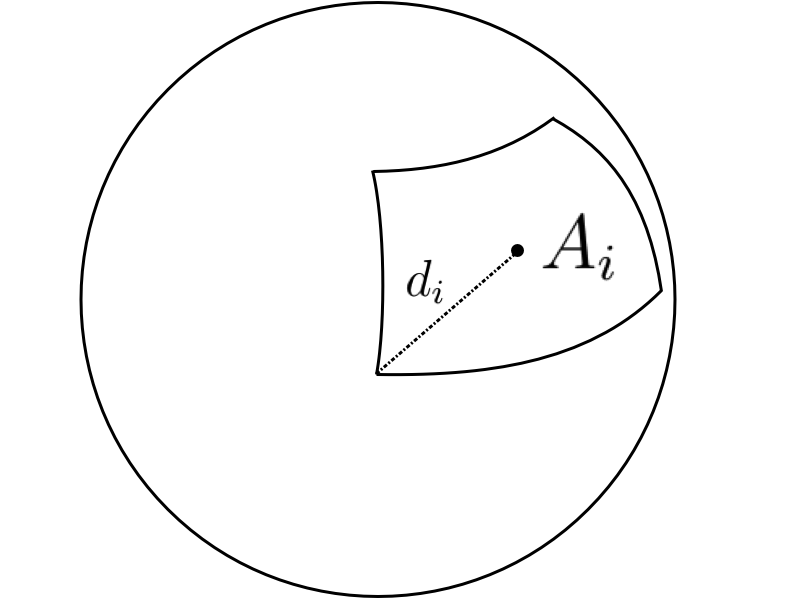
\includegraphics[width=0.4\linewidth]{figs/chapter1/d_iA_i.png}
	\captionof{figure}{Geometric characteristics of the i-th patch}
	\label{fig:Geometric characteristics of a patch}
\end{minipage}%
\begin{minipage}{.5\textwidth}
	\centering
	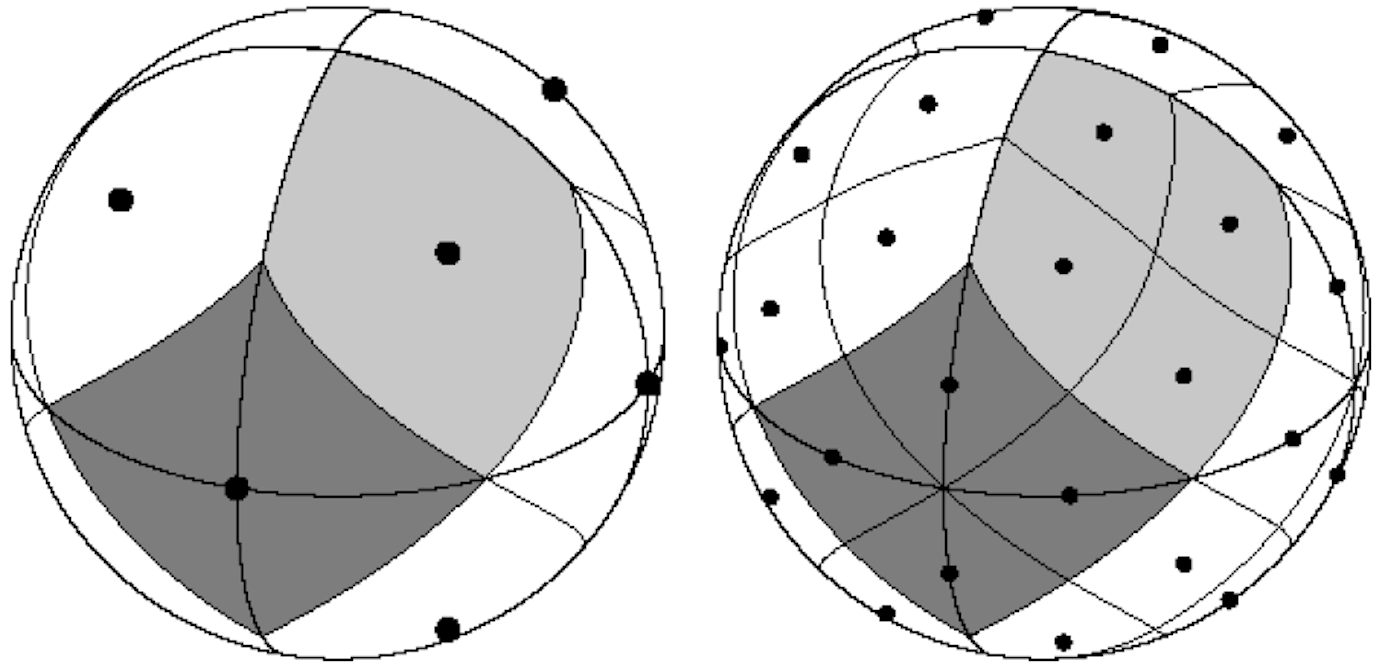
\includegraphics[width=0.7\linewidth]{figs/chapter1/Heal_Base.png}
	\captionof{figure}{HEALPix equal areas patches for $N_{side}=1$, $N_{side}=2$}
	\label{fig:HEALPix equal areas patches}
	\vspace{0.5cm}
\end{minipage}

It is interesting to notice these regularity conditions for the following reasons: in \cite{Belkin:2005:TTF:2138147.2138189} the sampling is drawn form a uniform random distribution on the sphere, and their proof heavily relies on the uniformity properties of the distribution from which the sampling is drawn. In our case the sampling is deterministic, and the fact that for a sphere there doesn't exist a regular sampling with more than 12 points (being the only regular samplings of the sphere the vertices of the Platonic solids) is indeed a problem that we need to overcome someway by imposing the regularity conditions above. 

\subsubsection{Point wise convergence of the Graph Laplacian in the HEALPix case}

As an intermediate result to the main result proved in Theorem \ref{theo:pointwise convergence in the healpix case}, our first goal is to prove that 
\vspace{0.5cm}
\begin{prop}\label{prop:1}
	For a sampling $\{x_i\in\mathcal S_2\}_{i=0}^{n-1}$ of the sphere, for all $f: \mathcal S_2 \rightarrow \mathbb R$ Lipschitz with respect to the euclidean distance $||\cdot||$, for all $y\in\mathcal S_2$, the Heat Kernel Graph Laplacian operator $L^t_n$ converges pointwise to the functional approximation of the Laplace Beltrami operator $L^t$
	$$ L_n^tf(y)\xrightarrow{n\to\infty} L^tf(y)$$
\end{prop} 
\vspace{0.5cm}


\begin{proof}
	We know by construction that the HEALPix sampling cut the sphere into equal areas. Given a HEALPix sampling $\{x_i\in\mathcal S_2\}_{i=0}^{n-1},\ n=12N^2,\ N=2^k,\ k\in\mathbb N$, we can define $S_n: \ |A_i|=S_n=\frac{|\mathcal S_2|}{n}\ \forall i=1, ..., n$ and $d_n := \max_{i=1,...n}d_i$.
	Let us assume that the function $f$ is Lipschitz with Lipschitz constant $\mathcal L_f$, we have 
	
	$$\left| \int_{A_{i}}f({\bf x})\text{d}{\mu(x)} - \frac{1}{n}f(\mathbf x_i)\right| \leq \mathcal L_fd_{n}\frac{1}{n} $$

	So, by triangular inequality and by summing all the contributions of all the $n$ patches $A_i$
	$$\left| \int_{\mathcal S_2}f({\bf x})\text{d}{\mu(x)} - \frac{1}{n}\sum_i f(\mathbf x_i)\right| \leq \sum_i \left| \int_{A_{i}}f({\bf x})\text{d}{\mu(x)} - \frac{1}{n}f(\mathbf x_i)\right|\leq n  \mathcal L_fd_{n}\frac{1}{n} = \mathcal L_fd_{n}$$	
	Thanks to this result, we have the following two pointwise convergences
	
	$$\forall f \text{ Lipschiz,}\quad \forall y\in\mathcal S_2,  \quad\quad \frac{1}{n}\sum_i e^{-\frac{||x_i-y||^2}{4t}}\rightarrow \int e^{-\frac{||x-y||^2}{4t}}d\mu(x)$$
	$$\forall f \text{ Lipschiz,}\quad \forall y\in\mathcal S_2,  \quad\quad \frac{1}{n}\sum_i e^{-\frac{||x_i-y||^2}{4t}}f(x_i)\rightarrow \int e^{-\frac{||x-y||^2}{4t}}f(x)d\mu(x)$$
	
	Together with definitions \ref{def:Heat Kernel Graph Laplacian operator} and \ref{def:Functional approximation to the Laplace-Beltrami operator} this end the proof.
\end{proof}
\vspace{0.5cm}

Now, we just proved that \textit{keeping t fixed} $L_n^tf(x)\rightarrow L^tf(x)$. Now our goal is to prove that:

\vspace{0.5cm}
\begin{prop}\label{prop:2}
$$\left|\frac{1}{4\pi t^2}\left(L_n^tf(x) -L^tf(x)\right)\right|\xrightarrow[n\to \infty]{t\to 0}0$$
\textit{for $t\to0$ and $n\to\infty$ at the same time}. In other words, there exists a sequence $(t_n), \\ \lim_{n\to\infty}t_n=0$ such that 
$$\forall f \text{ Lipschitz, } \forall x\in\mathcal S_2 \quad \left|\frac{1}{4\pi t_n^2}\left(L_n^{t_n}f(x) - L^{t_n}f(x)\right)\right|\xrightarrow{n\to \infty}0$$
\end{prop}
\vspace{0.5cm}

The main result of this section, theorem  \ref{theo:pointwise convergence in the healpix case}, is then an immediate consequence of Proposition \ref{prop:2} and Proposition \ref{prop:3}.


\begin{proof}
	
	We define for simplicity of notation
	$$\phi^t(x;y) := e^{-\frac{||x-y||^2}{4t}}\left(f(y)-f(x)\right)$$
	$$K^t(x,y) :=  e^{-\frac{||x-y||^2}{4t}}$$

	
	we start by writing the following chain of inequalities
	$$||L_n^tf-L^tf||_\infty = \max _{y\in \mathcal S_2} \left|L_n^tf(y)-L^tf(y)\right|=$$
	$$= \max _{y\in \mathcal S_2} \left| \frac{1}{n} \sum_{i=1}^n \phi^t(x_i; y)- \int_{\mathcal S_2} \phi^t(x;y)d\mu(x) \right|$$
	$$\leq \max _{y\in \mathcal S_2}  \sum_{i=1}^n   \left| \frac{1}{n}  \phi^t(x_i; y)- \int_{A_i} \phi^t(x;y)d\mu(x) \right|$$

	$$\leq  \max _{y\in \mathcal S_2} \left[\mathcal L_{\phi^t_y}d_n \right]$$
	
	where $\mathcal L_{\phi^t_y}$ is the Lipschitz constant of $x \rightarrow \phi^t(x, y)$ and where we used for the last inequality the arguments used in Step 1. If we assume $d_n\leq \frac{C}{\sqrt{n}}$ and remember that for HEALPix $n=12N^2$ we have that
	
	$$||L_n^tf-L^tf||_\infty  \leq  \max _{y\in \mathcal S_2} \left[ \mathcal L_{\phi^t_y} \frac{C}{N} \right]$$
	
	Let's now find the explicit dependence $t\rightarrow \mathcal L_{\phi^t_y}$
	
	$\mathcal L_{\phi^t_y} = ||\partial_x\phi^t(x;y)||_\infty = ||\partial_x\left(K^t(x;y)f(x)\right)||_\infty = ||\partial_x K^t(x;y)f(x) + K^t(x;y)\partial_x f(x)||_\infty \leq$
	
	$ \leq ||\partial_x K^t(x;y)f(x)||_\infty + ||K^t(x;y)\partial_x f(x)||_\infty \leq  ||\partial_x K^t(x;y)||_\infty||f(x)||_\infty + ||K^t(x;y)||_\infty||\partial_x f(x)||_\infty = $
	
	$ = ||\partial_x K^t(x;y)||_\infty||f(x)||_\infty + ||\partial_x f(x)||_\infty = \mathcal L_{K^t_y} ||f||_\infty + ||\partial_xf||_\infty = \mathcal L_{K^t_y} ||f||_\infty + \mathcal L_f$
	
	where $\mathcal L_{K^t_y}$ is the Lipschitz constant of $x\rightarrow K^t(x;y)$. We can observe that such constant does not depend on $y$. Thus
	
	$\mathcal L_{K^t_y} = \norm{\partial_x e^{-\frac{x^2}{4t}}}_\infty = \norm{\frac{x}{2t}e^{-\frac{x^2}{4t}}}_\infty = \left. \frac{x}{2t}e^{-\frac{x^2}{4t}}\right|_{x=\sqrt{2t}}=(2et)^{-\frac{1}{2}}\propto t ^ {-\frac{1}{2}}$
	
	So we can continue
	
	$$ \max _{y\in \mathcal S_2} \left[  \mathcal L_{\phi^t_y} \frac{C}{N} \right]\leq$$
	$$ \leq \left[   \frac{C}{N} \left( (2et)^{-\frac{1}{2}} \norm{f}_\infty + \mathcal L_f \right)\right]\leq$$
	$$  \leq \frac{C\norm{f}_\infty}{N(2et)^\frac{1}{2}} +   \frac{C}{N}\mathcal L_f$$
	
	So we have that, rescaling by a factor $\frac{1}{4\pi t^2}$
	
	$$\norm{\frac{1}{4\pi t^2}\left(L_n^tf-L^tf\right)}_\infty\leq$$
	$$\leq \frac{1}{4\pi t^2}\norm{\left(L_n^tf-L^tf\right)}_\infty \leq$$
	$$ \leq \frac{C}{4\pi}\left[\frac{\norm{f}_\infty}{\sqrt{2e}}\frac{1}{Nt^\frac{5}{2}} + \frac{\mathcal L_f}{Nt^2}\right]$$
	
	we want $\begin{cases}
	t \rightarrow 0\\
	N \rightarrow \infty\\
	Nt^\frac{5}{2} \rightarrow \infty\\
	Nt^2 \rightarrow \infty
	\end{cases}$ in order for $ \frac{C}{4\pi}\left[\frac{\norm{f}_\infty}{\sqrt{2e}}\frac{1}{Nt^\frac{5}{2}} + \frac{\mathcal L_f}{Nt^2}\right] \xrightarrow[t\to 0 ]{N\to\infty}0$
	
	This is true if $\begin{cases}
	t(N) = N^\beta, &\beta\in(-\frac{2}{5}, 0) \\
	t(N) = N^\beta, &\beta\in(-\frac{1}{2}, 0)
	\end{cases} \implies t(N) = N^\beta, \quad \beta\in(-\frac{2}{5}, 0)$
	
	Indeed 
	
	$Nt^\frac{5}{2}=N^{\frac{5}{2}\beta+1}\xrightarrow{N \to \infty} \infty$ since $\frac{5}{2}\beta+1>0 \iff \beta>-\frac{2}{5}$
	
	$Nt^2=N^{2\beta+1}\xrightarrow {N \to \infty} \infty$ since $2\beta+1>0 \iff \beta>-\frac{1}{2}$
	
	So, for $t=N^\beta$ with $\beta\in(-\frac{2}{5}, 0)$ we have that 
	
	$$\begin{cases}
	(t_N)\xrightarrow{N\to\infty}0\\
	\norm{\frac{1}{4\pi t_N^2}L_n^{t_N}f-\frac{1}{4\pi t_N^2}L^{t_N}f}_\infty  \xrightarrow{N\to\infty}0
	\end{cases}$$
	
\end{proof}

The proof of theorem \ref{theo:pointwise convergence in the healpix case} is now trivial:
\begin{proof}
	Thanks to Proposition \ref{prop:2} and Proposition \ref{prop:3}	we conclude that $\forall y\in\mathcal S_2 $
	$$\lim_{N\to\infty}\frac{1}{4\pi t_N^2} L_n^{t_N}f(y) =  \lim_{N\to\infty}\frac{1}{4\pi t_N^2} L^{t_N}f(y) = \frac{1}{|\mathcal S_2|}\triangle_{\mathcal S_2}f(y) $$
\end{proof}

[Final considerations]
We can see that the result obtained has the same form than the result obtained in \cite{Belkin:2005:TTF:2138147.2138189}. If Belkin et al. proved convergence in the random case for $\beta \in (-\frac{1}{4}, 0)$, we proved convergence in the HEALPix case for $\beta \in (-\frac{2}{5}, 0)$. This kind of result can be interpreted in the following way. In order to have convergence, we need to reduce the kernel width but \textit{not so fast} compared to the resolution of the graph. In other words, the kernel width has to be reduced but is somewhat limited by the resolution of the graph, that has to increase faster than $t^\frac{2}{5}$ goes to $0$.\\
\begin{remark}
	Note that this pointwise convergence do not impy spectral convergence! However it's a first step. 
\end{remark}
\subsection{How to build a better graph}
Current state of the art: DeepSphere.
Problems: we don't see the convergence expected. in figure \ref{fig:DeepSphere} we see that as $N_{side}$ grows, the eigenspaces of the graph Laplacian do not get more and more aligned with the eigenspaces spanned by the spherical harmonics, as we expected. Why? The parameters to choose are the following: the standard deviation of the Gaussian kernel $t$ and the number of neighbors of the graph. We'll see that the main cause of this bad behavior is the fixed number of neighbors used in \cite{DeepSphere} for the construction of the graph. We'll see that to obtain the desired convergence it is necessary to increase the number of neighbors as we decrease sigma, as we can show hereunder.
\begin{figure}[h]
	\label{fig:DeepSphere}
	\caption{Results from DeepSphere}
	\centering
	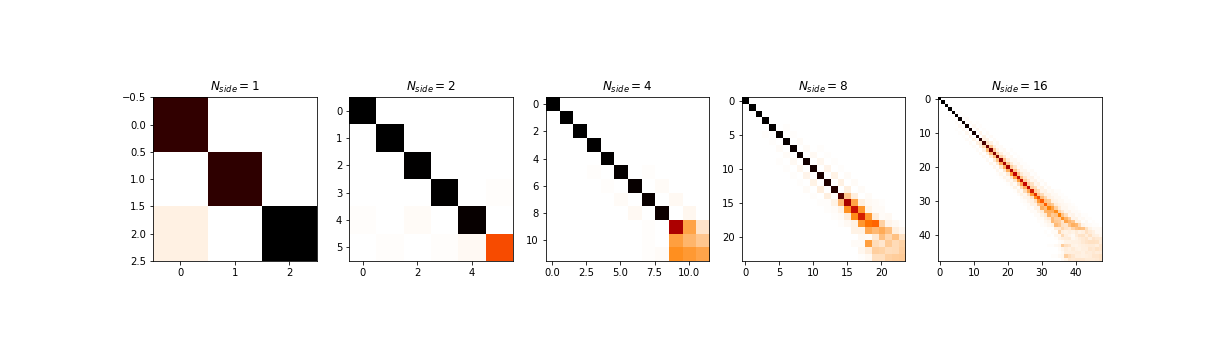
\includegraphics[width=0.9\textwidth]{../codes/02.HeatKernelGraphLaplacian/HEALPix/06_figures/deepsphere_original.png}
	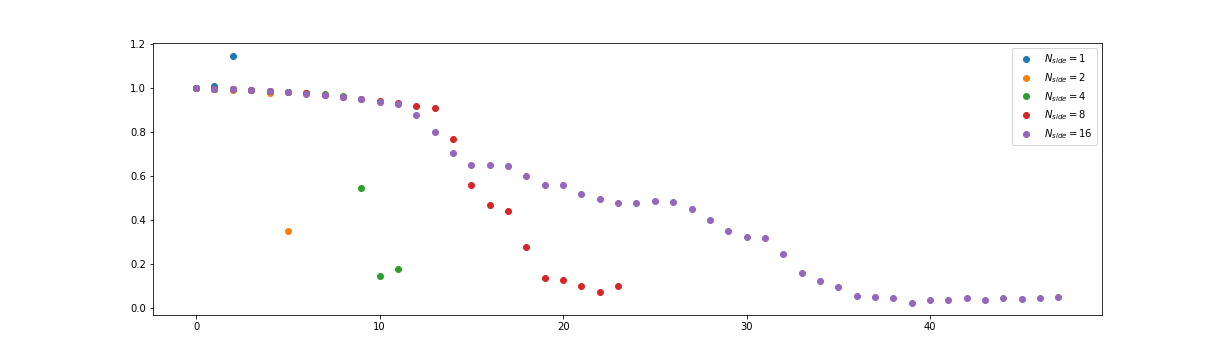
\includegraphics[width=0.9\textwidth]{../codes/02.HeatKernelGraphLaplacian/HEALPix/06_figures/deepsphere_original_diagonal.png}	
\end{figure}
\subsubsection{About the kernel width $t$}
Intuition: with a big $t$, the kernel is very wide and the graph can not distinguish the high frequencies. In other words, if we build a radius graph with $d=\bar d$ and connect all the neighbors of a node with the same weights $w$, all the variations on those nodes are indistinguishable. thus, above a certain frequency where the variations reach a wavelength $\omega \leq \bar d$, any graph operator would be blind to such frequencies (indeed, any reordering of the signal on the neighbors would lead to the same result). Thus, if we want our graph Laplacian to be able to distinguish such frequencies, we need our weight to change significantly in a short radius, that means \textbf{setting a $t$ of the order of magnitude of the nearest neighbors of a node}. This intuition was already used in DeepSphere. 

Remember that the convergence result proved in the previous section is valid for a full graph: let's try to see how a full graph built with the same values of $t$ used in \cite{DeepSphere} behaves. 
In figure \ref{fig:DeepSphere_full} we see how for such a full graph it is indeed possible to observe the expected convergence:
\begin{figure}[h]
	\label{fig:DeepSphere_full}
	\caption{DeepSphere \textbf{full}}
	\centering
	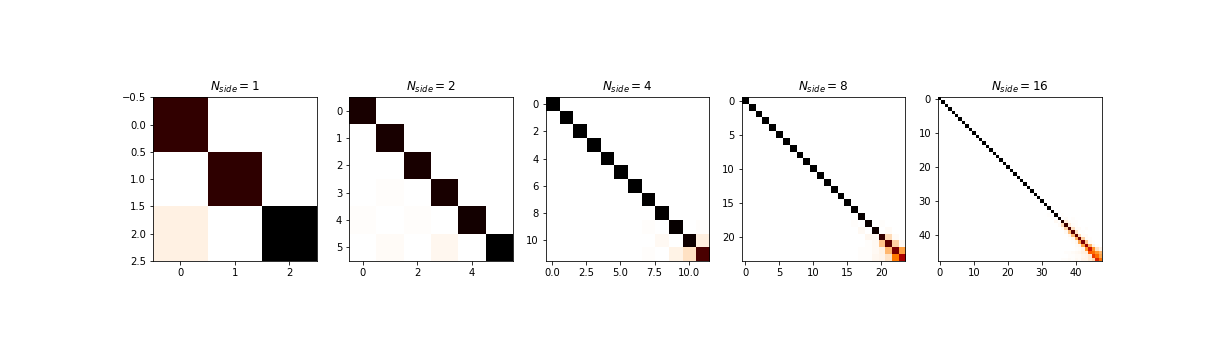
\includegraphics[width=0.9\textwidth]{../codes/02.HeatKernelGraphLaplacian/HEALPix/06_figures/deepsphere_full.png}
	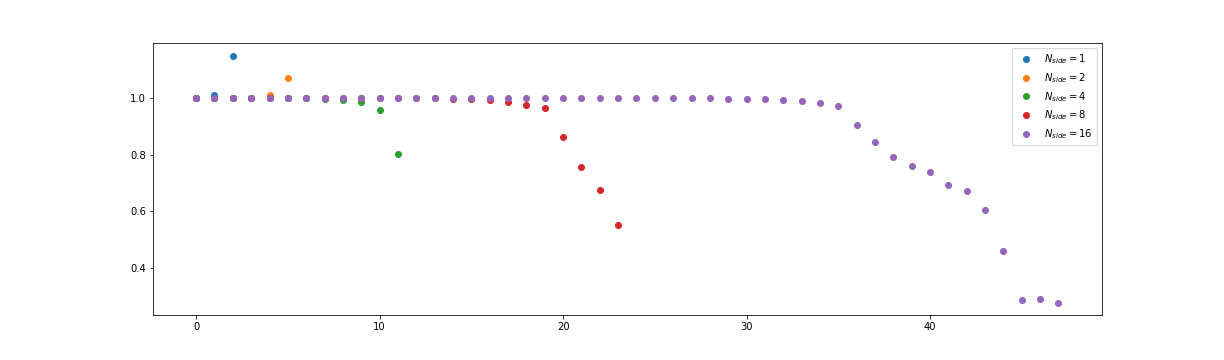
\includegraphics[width=0.9\textwidth]{../codes/02.HeatKernelGraphLaplacian/HEALPix/06_figures/deepsphere_full_diagonal.png}	
\end{figure}
A quick heuristic grid search has been used to find the following optimal parameters for different values of $N_{side}$ in the case of a full graph. The results are shown in figure \ref{fig:t}. We can see that the heuristic way of \cite{DeepSphere} of setting the standard deviation $t$ produces results very close to the optimal value.

\begin{figure}[h]
	\label{fig:t}
	\caption{Standard deviation of the Gaussian kernel  in a loglog plot. A straigh line indicates a polynomial relation.}
	\centering
	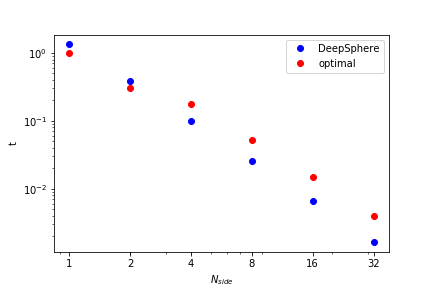
\includegraphics[width=0.5\textwidth]{../codes/02.HeatKernelGraphLaplacian/HEALPix/06_figures/kernelwidth.png}
\end{figure}

However, it is worth showing how the spectrum of the graph is sensible to such parameter. In figure \ref{fig:t_sensitity} it is shown how of the alignment of the eigenspaces is sensible to small changes of $t$. To produce this image $N_{side}$ was set to 16, and a full graph has been build where $t$ has been set first equal to the one used in \cite{DeepSphere} ($t=0.00647$) and then to the optimal value obtained in this work $t=0.015$.

\begin{figure}[h]
	\label{fig:t_sensitity}
	\caption{Standard deviation of the Gaussian kernel}
	\centering
	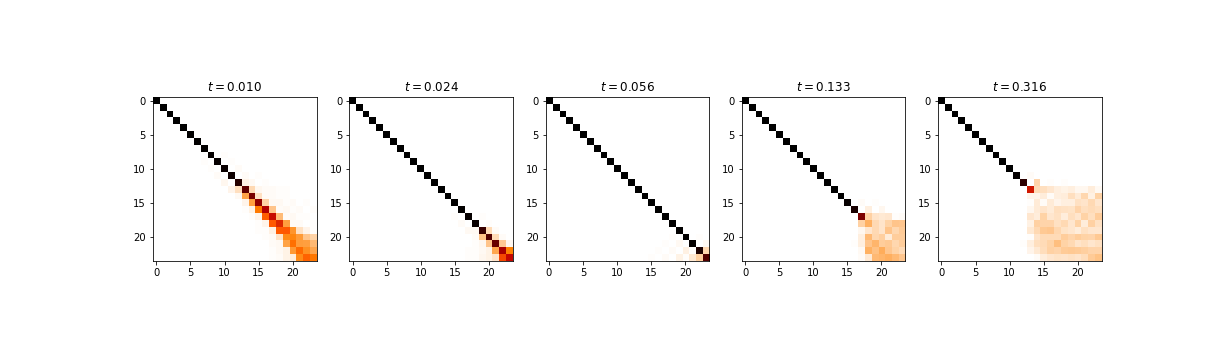
\includegraphics[width=0.9\textwidth]{../codes/02.HeatKernelGraphLaplacian/HEALPix/06_figures/t_sensitivity.png}
	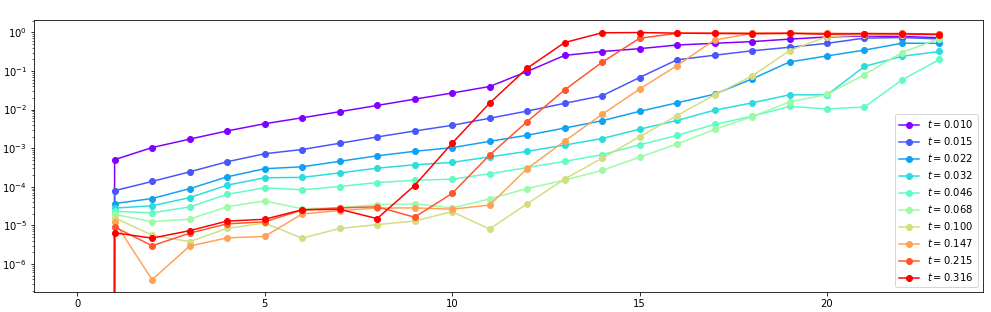
\includegraphics[width=0.9\textwidth]{../codes/02.HeatKernelGraphLaplacian/HEALPix/06_figures/t_sensitivity_diagonal.png}
\end{figure}

\subsubsection{Reducing the number of neighbors}
For what it concerns how to make the graph sparse, the intuition is the following: remember that we want our graph Laplacian to approximate the operator $L^t$
$$\frac{1}{n}\left(\sum_i e^{-\frac{||x_i-y||^2}{4t}}(f(y)-f(x_i)) \right) \approx \frac{1}{ 4\pi}\int_\mathcal M e^{-\frac{||x-y||^2}{4t}}\left(f(y)-f(x)\right)d\mu(x) $$

However, with a full graph the operation of filtering with a polynomial of the graph Laplacian would cost $\mathcal O (n^2)$, same order of magnitude of the method proposed in \cite{bibid}. We want a method to make the graph sparse such that the number of non-null entries of the Laplacian is linear $\mathcal O (n)$, making the filtering operation $f\rightarrow \mathcal P(L)f$ linear in the number of pixels. Deferrard et al. \cite{bibid} fixed the number of neighbors to 7/8. However, their results do not show the expected spectral convergence.
Making the graph sparse means approximating some weights $w_{i,j}=e^{-\frac{||x_i-x_j||^2}{4t}} \approx 0$. For this to be accurate we need those weights to be close to 0. A method to be sure that the approximation isn't too bad is the following: \textbf{instead of fixing the number of neighbors, fixing a threshold $k$ on $w_{i,j}=e^{-\frac{||x_i-x_j||^2}{4t}}$ such that} 

$$w_{i,j} = \begin{cases}
e^{-\frac{||x_i-x_j||^2}{4t}}\quad& \text{if } e^{-\frac{||x_i-x_j||^2}{4t}} \geq k\\
0 \quad & \text{if } e^{-\frac{||x_i-x_j||^2}{4t}} < k
\end{cases}$$

By setting $k = 0.01$ here's the results:

\begin{center}
	\begin{tabular}{ c|c} 
		
		$N_{side}$ & Number of neighbors \\ 
		
		1 & 11 \\ 
		2 & 16 \\ 
		4 & 37 \\ 
		8 & 43 \\ 
		16 & 52 \\ 
		
	\end{tabular}
\end{center}

\begin{figure}[h]
	\label{fig:DeepSphere_thresholded}
	\caption{Deepsphere \textbf{thresholded at $k=0.01$}}
	\centering
	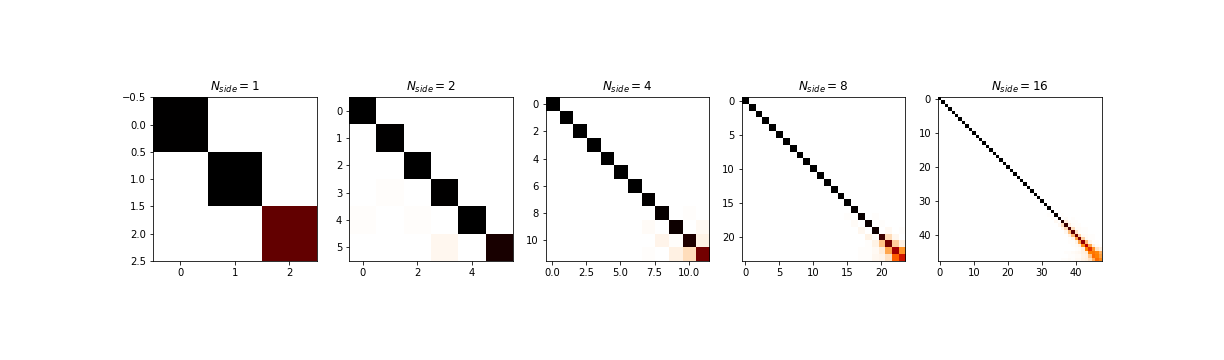
\includegraphics[width=0.9\textwidth]{../codes/02.HeatKernelGraphLaplacian/HEALPix/06_figures/deepsphere_thresholded.png}	
	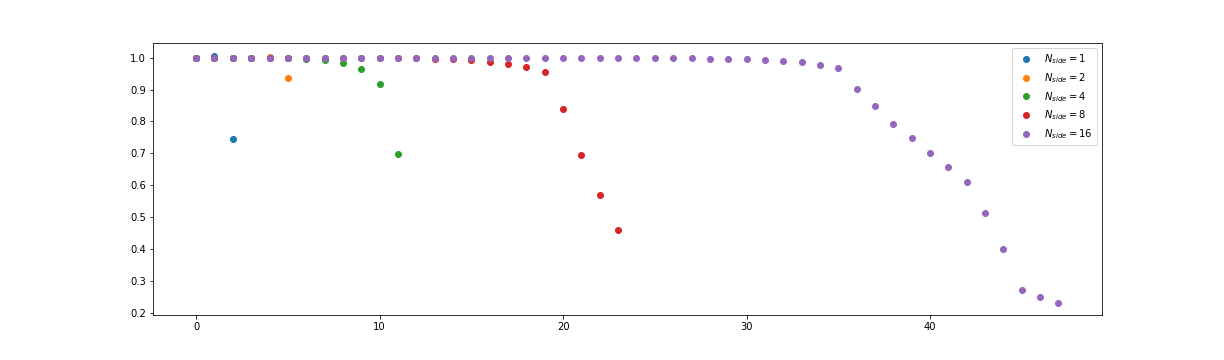
\includegraphics[width=0.9\textwidth]{../codes/02.HeatKernelGraphLaplacian/HEALPix/06_figures/deepsphere_thresholded_diagonal.png}	
\end{figure}

We see that to keep the threshold fixed we need to increase the number of neighbors as $N_{side}$ gets bigger. Again, the intuition is the following: to have spectral convergence (a strong type of convergence) we need more and more global information and more precise. 
\subsection{Experimental validation}
Here we report Frederick's results with the two different constructions
